\chapter{Executive Summary }
\label{ch:project-overview}
\section{Overview}

The Deep Underground Neutrino Experiment (DUNE) will be a world-class neutrino observatory and nucleon decay detector designed to answer fundamental questions about the nature of elemen- tary particles and their role in the universe. The international DUNE experiment, hosted by the U.S. Department of Energy's \fnal in Illinois, will consist of a far detector to be located about \SI{1.5}{km} underground at the Sanford Underground Research Facility (\surf) in South Dakota, USA, at a distance of  \SI{1300}{\km} from \fnal{}, and a near detector to be located at \fnal. The far detector will be a very large, modular liquid argon time-projection chamber (\lartpc) with a \fdfiducialmass (\SI{40}{\giga\gram}). This \lar technology will make it possible to reconstruct neutrino interactions with image-like precision and unprecedented resolution. 

The far detector will be exposed to the world's most intense neutrino beam originating at \fnal{}. A high-precision near detector, located \SI{575}{m} from the neutrino source on the \fnal site, will be used to characterize the intensity and energy spectrum of this wide-band beam. The Long-Baseline Neutrino Facility (LBNF), also hosted by \fnal, provides the infrastructure for this complex system of detectors at the Illinois and South Dakota sites. LBNF assumes the responsibility for the neutrino beam, the deep-underground site, and the infrastructure for the DUNE detectors. 


\begin{dunefigure}[DUNE collaboration global map]{fig:mhexec}{The international DUNE
collaboration. Countries with DUNE membership are shown in orange.}
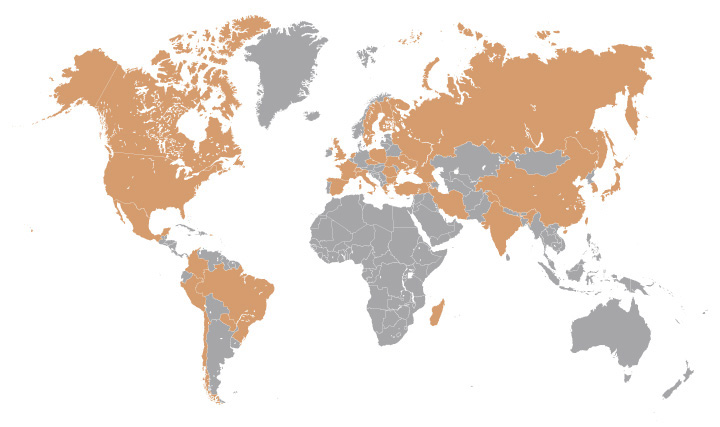
\includegraphics[width=0.9\textwidth]{global.jpg}
\label{fig:map}
\end{dunefigure}

The DUNE collaboration is a truly global organization including more than \num{1000} scientists and engineers from \num{32} countries (Figure~\ref{fig:map}). It represents the culmination of several worldwide efforts that developed independent paths toward a next-generation long-baseline (LBL) neutrino experiment over the last decade. It was formed in April 2015, combining the strengths of the LBNE project in the USA and the LBNO project in Europe, adding many new international partners in the process. DUNE thus represents the convergence of a substantial fraction of the worldwide neutrino-physics community around the opportunity provided by the large investment planned by the U.S. Department of Energy (DOE) and \fnal to support a significant expansion of the underground infrastructure at \surf in South Dakota, and to create a megawatt neutrino-beam facility at \fnal by 2026. The Proton Improvement Plan-II (PIP-II) upgrade at \fnal~\cite{pip2-2013} will enable the accelerator to drive the new neutrino beamline with a \SI{80}{\GeV} primary proton beam at a beam power %from \SI{1.07}{\MW} 
up to \pipiibeampower{}. A further planned upgrade 
of the accelerator complex will enable it to provide up to \SI{2.4}{\MW} of beam power by 2030. 

The LBNF/DUNE project (the \textit{project}) strategy presented in this technical proposal has been developed to meet the requirements set out in the report of the Particle Physics Project Prioritization Panel (P5 in 2014). It also takes into account the recommendations of the European Strategy for Particle  Physics (ESPP) adopted by the CERN Council in 2013, which classified the \dword{lbl} neutrino program as one of the four scientific objectives that require international infrastructure.
%which recommends development of
%a program to pave the way for a substantial European role in future long-%baseline experiments.

The P5 report~\cite{p5report} set the goal of reaching a sensitivity to \dword{cpv} of better than three standard deviations (\num{3}$\sigma$) over more than $75\%$ 
of the range of possible values of the unknown \dshort{cp}-violating phase \deltacp.
Based partly on this goal, they stated that ``the 
minimum requirements to proceed are the identified capability to reach an exposure 
of \num{120}~\ktMWyr{} by the 2035 time frame, the far detector situated underground 
with cavern space for expansion to at least \fdfiducialmass \lar fiducial volume, and \SI{1.2}{MW} 
beam power upgradeable to multi-megawatt power.
The experiment should have the demonstrated 
capability to search for \dwords{snb} and for proton decay, providing a significant 
improvement in discovery sensitivity over current searches for the proton lifetime.'' The strategy and design presented in this technical proposal meet these requirements.
%Based on the resource-loaded schedules for the reference designs of the facility %(\vollbnf)
%and the detectors, %(\voldune), 
%the strategy presented here meets these criteria. 


This document serves as the \dword{tp} for the DUNE \dword{fd}.  The \dword{tp}  is intended to provide a clear statement of the physics goals and methods of the DUNE experiment, and to describe the detector technologies that have been designed to achieve these goals. Introductions to each chapter are intended to be useful and informative to technical specialists who serve in national science agencies. The body of the document is intended to be useful and informative to members of the international high energy physics community.  The \dword{tp} deliberately emphasizes the connections between the physics and technologies of the DUNE \dword{fd} modules. Very important project related tasks are presented in summary form. No information about cost is included, and schedule information appears only in the form of high-level milestones. The \dword{tp} forms the nucleus of the \dword{tdr}, which will be presented to international science  agencies and the high energy physics (HEP) community in 2019.

%Volumes 2 and 3 of the TP provide detailed descriptions of the single phase and dual phase TPC options respectively.  These volumes have been prepared by the appropriated detector consortia with input from the DUNE Technical Coordinator team.  Volume 1, this volume, contains, in addition to this executive summary, chapters that describe the DUNE physics program and two overarching systems required to execute this program: computing and calibration.

%

%%%%%%%%%%%%%%%%%%%%%%%%%%%%%%%%%%%%%%%%%%%%%%%%%%%%%%%%%%%%%%%%
\section{Primary Science Goals} % (Ed)}


The DUNE experiment will combine the world's most intense neutrino beam, a deep underground site, and massive LAr detectors to enable a broad science program addressing some of the most fundamental questions in particle physics. 

%Searches for CP violation in neutrino oscillations may give insight into the origin of the matter-antimatter asymmetry, one of the fundamental questions in particle physics and cosmology. Detection of neutrinos from a nearby supernova could provide a wealth of information about neutrinos and the dynamics of supernovae. Observation of proton decay would dramatically change our understanding of particle physics

The primary science goals of DUNE, described in detail in Chapter~\ref{ch:exec-summ-physics}, are to: 
\begin{itemize}

\item Carry out a comprehensive program of neutrino oscillation measurements using \numu and \anumu beams from \fnal. This program includes measurements of the \dword{cp} phase, determination of the neutrino mass ordering (the sign of \dm{31}$ \equiv m_3^2-m_1^2$), measurement of the mixing angle $\theta_{23}$ and the determination of the octant in which this angle lies,
and sensitive tests of the three-neutrino paradigm. Paramount among these is the search for \dword{cpv} in neutrino oscillations, which may give insight into the origin of the matter-antimatter asymmetry, one of the fundamental questions in particle physics and cosmology. 

\item Search for proton decay in several important decay modes. The observation of proton decay would represent a ground-breaking discovery in physics, providing a key requirement for grand unification of the forces. 

    \item Detect and measure the $\nu_\text{e}$ flux from a core-collapse supernova within our galaxy, should one occur during the lifetime of the DUNE experiment. Such a measurement would provide a wealth of unique information about the early stages of core-collapse, and could even signal the birth of a black hole.
    
\end{itemize}

The intense neutrino beam from LBNF, the massive DUNE \lartpc far detector, and the high-resolution
DUNE near detector will also provide a rich ancillary science program, beyond the primary goals of the experiment. The ancillary science program includes
\begin{itemize}
     \item other accelerator-based neutrino flavor transition measurements with sensitivity to beyond the standard model (BSM) physics, such as non-standard interactions (NSIs), \dword{cpt} violation, sterile neutrinos, large extra dimensions, heavy neutral leptons;
 and measurements of tau neutrino appearance;
     \item measurements of neutrino oscillation phenomena using atmospheric neutrinos;
     \item a rich neutrino interaction physics program utilizing the DUNE near detector, including a wide-range of measurements of neutrino cross sections, studies of nuclear effects; %, including neutrino final-state interactions, measurements of the structure of nucleons, and  measurement of $\sin^2\theta_\text{W}$;
     \item  searches for dark matter.
\end{itemize} 
Further advancements in the \lartpc %far detector 
technology during the course of the DUNE far detector construction may open up the opportunity
to observe very low-energy phenomena such as solar neutrinos or even the diffuse supernova neutrino flux.


%%%%%%%%%%%%%%%%%%%%%%%%%%%%%%%%%%%%%%%%%%%%%%%%%%%%%%%%%%%%%%%
\section{The LBNF Facility} 

The Long-Baseline Neutrino
Facility (LBNF), hosted by Fermilab, is separate from the DUNE collaboration and is intended to enable the construction and operation of the DUNE detectors in South Dakota and Illinois.
The DUNE collaboration will construct a deep-underground neutrino observatory in South Dakota based on four independent \nominalmodsize \lartpc{}s. % at \surf. %the Sanford Underground Research Facility (\surf) in South Dakota.
LBNF will provide facilities in Illinois and South Dakota to enable the scientific program of DUNE.
These facilities are geographically separated into the near site facilities, those to be constructed
at \fnal, and the far site facilities, located at \surf. Figure~\ref{fig:lbnf} shows
a schematic of the facilities at the two sites, and Figure~\ref{fig:caverns} shows the cavern layout. 

\begin{dunefigure}[ 	
LBNF/DUNE project: beam from Illinois to South Dakota]{fig:lbnf}{ 	
LBNF/DUNE project: beam from Illinois to South Dakota.}
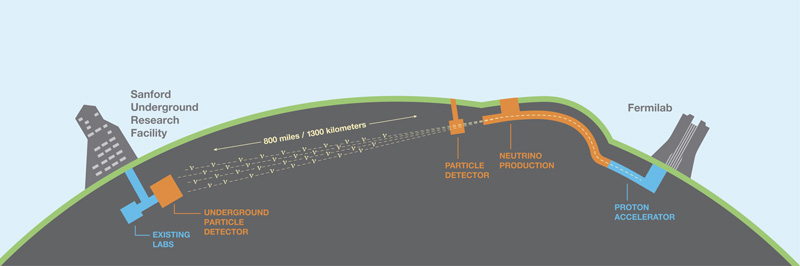
\includegraphics[width=0.9\textwidth]{lbnf_dune_graphic_miles_km-15-0031-01.jpg}
%\label{fig:mhexec}
\end{dunefigure}

Specifically, the Long-Baseline Neutrino Facility (LBNF) provides
\begin{itemize}

\item  the  technical and conventional facilities for a powerful \MWadj{1.2} neutrino beam utilizing the PIP-II upgrade of the \fnal accelerator 
complex, to become operational by \beamturnon  
at the latest, and to be upgradable to \SI{2.4}{\MW} with the proposed 
PIP-III upgrade;

\item  the civil construction, or \dword{cf}, for the near detector systems at \fnal; (see Figure~\ref{fig:beamline}); 

\item the excavation of four underground caverns at \surf, planned to be completed 
by 2021 
under a single contract, with each cavern to be capable of housing a cryostat with 
a minimum \nominalmodsize fiducial mass \lartpc; and



\item surface, shaft, and underground infrastructure to support 
the outfitting of the caverns with four free-standing, steel-supported cryostats 
and the required cryogenics systems. The first cryostat will be available for filling, after installation of the detector components, by
2023, enabling a rapid deployment of the first two \nominalmodsize far detector modules. 
The intention is to install the third and fourth cryostats as rapidly as funding will 
allow.

\end{itemize}

\begin{dunefigure}[ 	
Underground caverns for DUNE in South Dakota]{fig:caverns}{Underground caverns for DUNE far detectors and cryogenic systems at \surf{}, in South Dakota.}
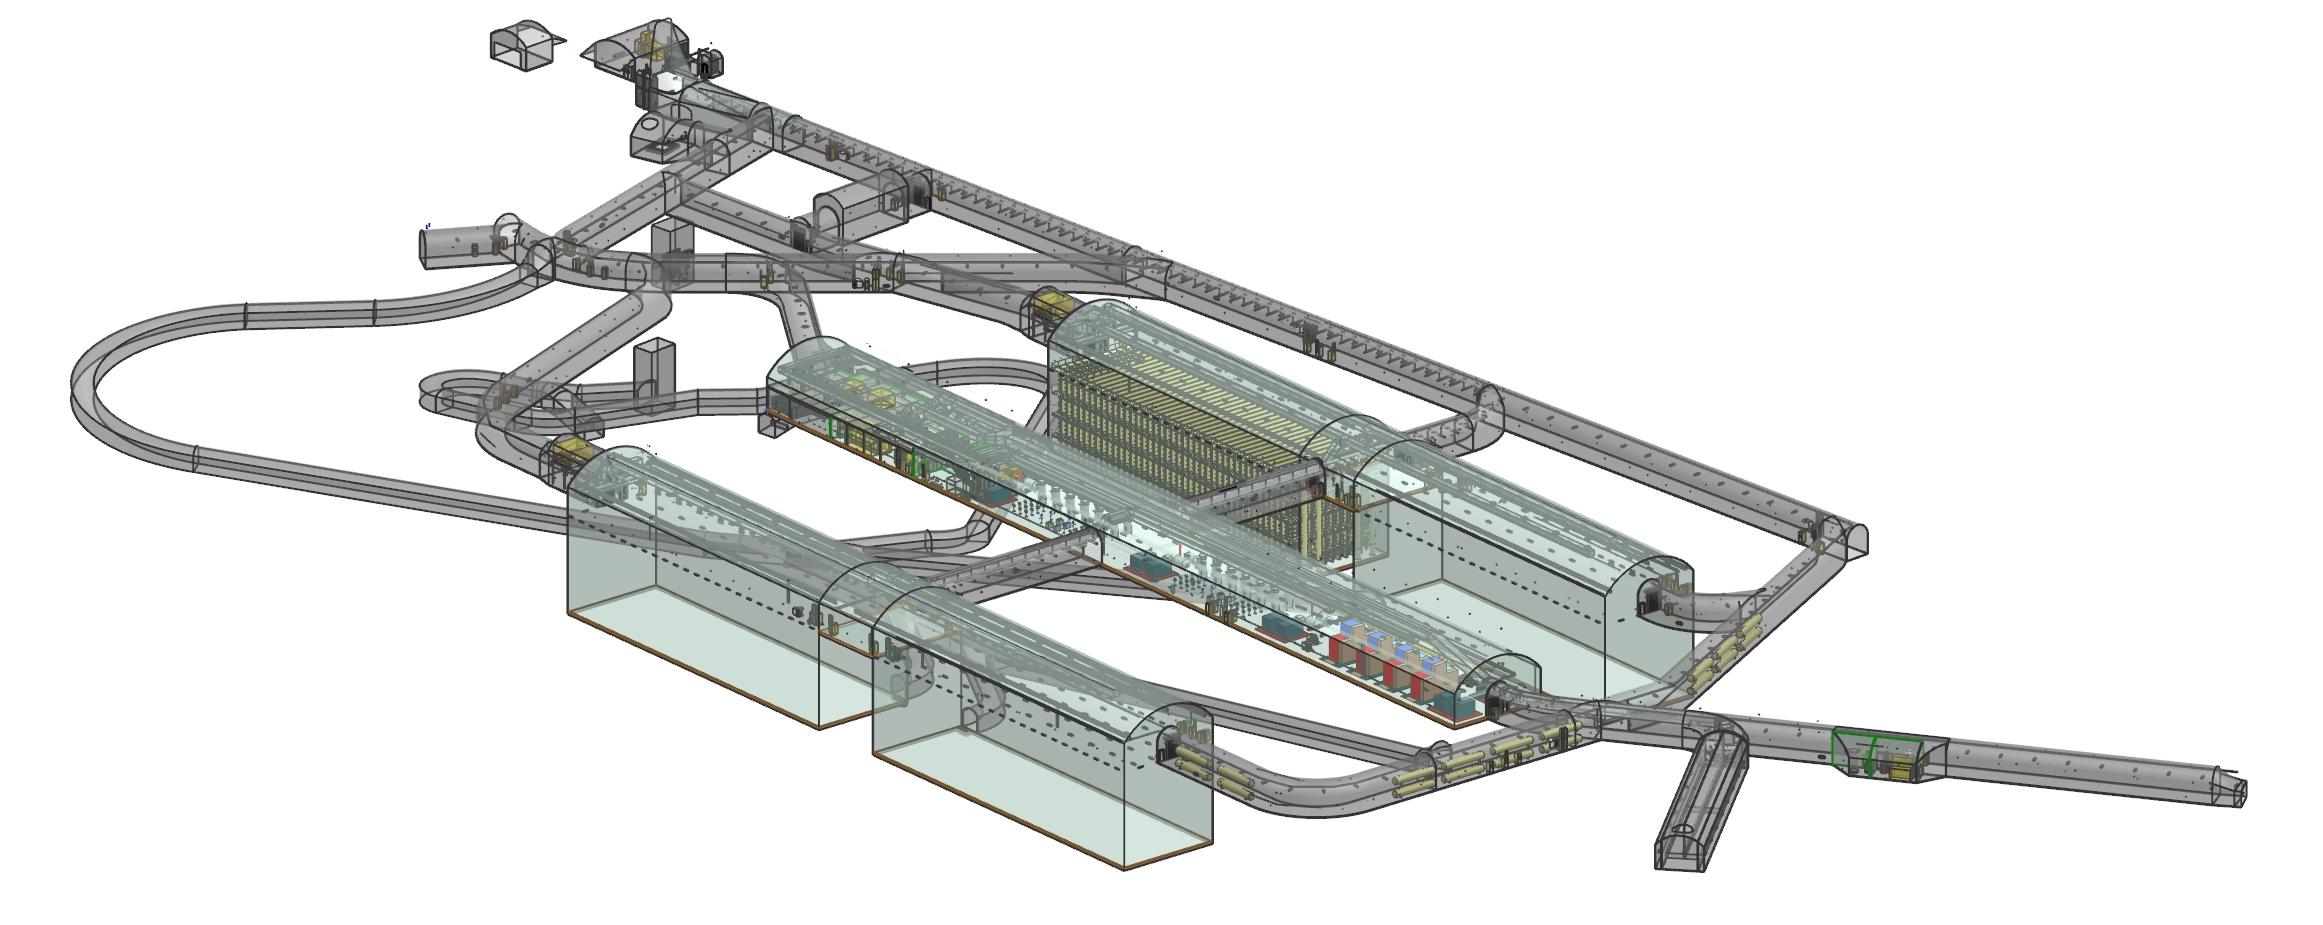
\includegraphics[width=0.95\textwidth]{far-detector-configuration-hi-res.jpeg}
\end{dunefigure}

\begin{dunefigure}[Neutrino beamline and DUNE near detector hall in Illinois
]{fig:beamline}{Neutrino beamline and DUNE near detector hall at Fermilab, in Illinois}
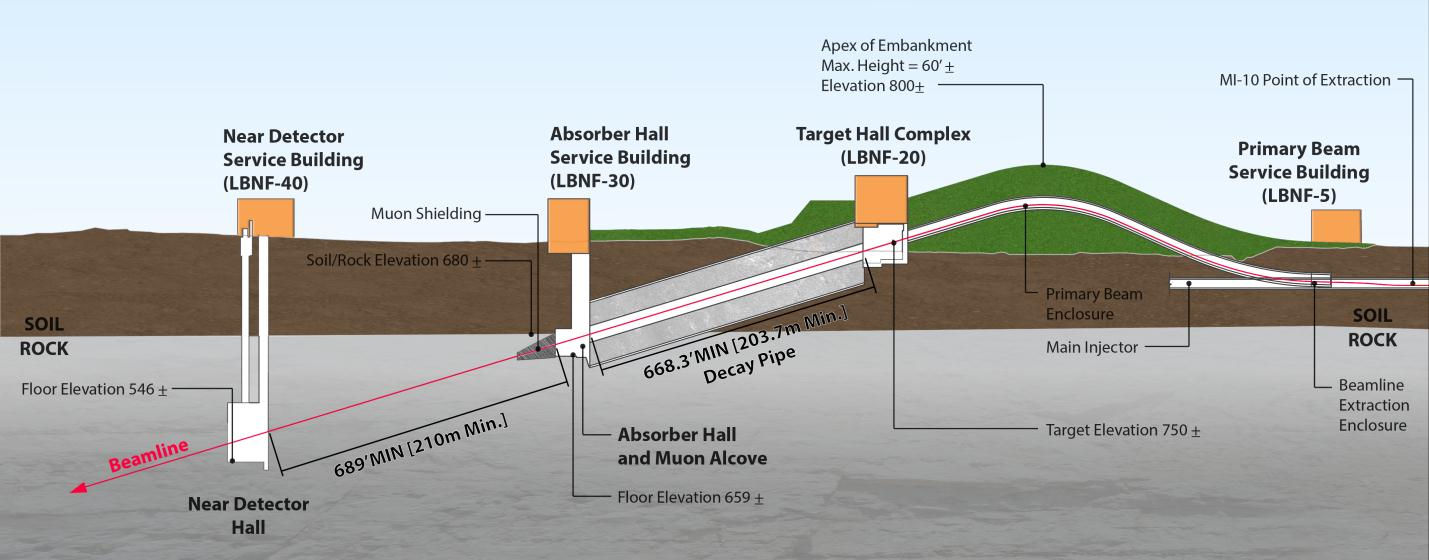
\includegraphics[width=0.95\textwidth]{figures/beamline-sideview.jpg}
\end{dunefigure}


The success of the DUNE project depends on the successful realization of the LBNF facilities.
This technical proposal focuses on the DUNE physics program that is enabled by
the first three \dword{fd} modules, which are expected to be based on the \dword{sp} and \dword{dp} \lar technologies. 

\section{The DUNE Experiment} %(Ed)}

% ecb: Do ProtoDUNEs show up here or in a separate section? Somewhere, we need to state what specific performance measures we are counting on having from ProtoDUNE before the TDR.

The DUNE experiment includes a precision near detector at the edge of the \fnal site, in Batavia, Illinois, and a very large, modular far detector about \SI{1.5}{km} underground at \surf in Lead, South Dakota, \SI{1300}{km} (\SI{800}{miles}) from \fnal. The DUNE far detector is the focus of this technical proposal. 

The near detector will be located \SI{575}{m} from the target. It will consist of a \lartpc followed by a fine-grained magnetic spectrometer. The \lartpc will use pixel readout to deal with the high occupancy from neutrino events in the intense LBNF beam. The details of the magnetic spectrometer will be resolved in the near future. The goal for the near detector group is to produce a \dword{cdr} at the time of the \dword{fd} \dword{tdr}. The near detector \dword{cdr} will provide information critical to establishing the physics reach for the primary neutrino oscillation program of DUNE. The near detector \dword{tdr} will follow the \dword{fd} \dword{tdr} by approximately one year, consistent with the near detector construction schedule.

The DUNE \dword{fd} will consist of four similar \lartpc{}s, each with fiducial mass of at least \nominalmodsize, installed about \SI{1.5}{km} underground. Each detector will be installed in a cryostat with internal dimensions
\cryostatwdth (W) $\times$ \cryostatht (H) $\times$ \cryostatlen (L), and will contain a total \lar{} mass of about \larmass{}.
The \lartpc technology provides
excellent tracking and calorimetry performance, making it an ideal
choice for the DUNE far detectors. The four identically sized cryostats give flexibility for staging and evolution of the \lartpc technology.

DUNE is planning for and prototyping two \lartpc technologies:
\begin{itemize}
\item Single-phase (SP): This technology was pioneered by the ICARUS project, and after several decades of worldwide R\&D, is now a mature technology. It is the technology used for \fnal{}'s currently operating \microboone, and the planned SBND. In the \single technology, ionization charges are drifted horizontally in \lar and read out on wires in the liquid. The maximum drift length in the DUNE \dword{spmod} is \spmaxdrift and the nominal drift field is \spmaxfield, corresponding to a total high voltage of \sptargetdriftvoltpos. There is no signal amplification in the liquid, so readout with good signal-to-noise requires very low-noise electronics.

\item Dual-phase (DP): This technology was pioneered at large scale by the \dword{wa105} collaboration. It is less established than the \single technology but offers a number of potential advantages and challenges. Here, ionization charges are drifted vertically in \lar and transferred into the gas above the liquid. The signal charges are then amplified in the gas phase using large electron multipliers (LEMs). This gain reduces the requirements on the electronics, and makes it possible for the \dword{dpmod} to have a longer drift, which requires a correspondingly higher voltage.
The maximum drift length in the \dword{dpmod} is \dpmaxdrift and the nominal drift field is \dpnominaldriftfield, corresponding to a total high voltage of \dptargetdriftvoltpos. 

\end{itemize}
The plans for the single and dual-phase TPCs are described in detail in Volumes 2 and 3 of this technical proposal.

The DUNE collaboration is committed to deploying both technologies. 
For planning purposes, DUNE assumes the first \dword{detmodule} to be
\single and the second to be \dual.
The actual sequence of \dword{detmodule} installation will depend on results from the prototype detectors, described below, and on available resources.


The collaboration is in now in the final stages of constructing two large prototype detectors (called \dwords{protodune}), one employing \single readout (\dword{pdsp}) and the other employing \dual readout (\dword{pddp}). Each is approximately one-twentieth of a DUNE \dword{detmodule}, but uses components identical in size to those of the full-scale module. \dword{pdsp} has the same \spmaxdrift maximum drift length as the full \dword{spmod}. \dword{pddp} has a \SI{6}{m} maximum drift length, half of that planned for the \dword{dpmod}. 

These large-scale prototypes will allow us to validate key aspects of the TPC designs, test engineering procedures, and collect valuable calibration data using a hadron test beam. The following list includes the key goals of the \dword{protodune} program:
\begin{enumerate}
\item Test production of components:
\begin{itemize}
\item stress testing of the production and quality
assurance processes of detector components,
\item mitigation of the associated risks for the far detector.
\end{itemize}
\item Validate installation procedures:
\begin{itemize}
\item test of the interfaces between the detector elements,
\item mitigation of the associated risks for the far detector.
\end{itemize}
\item Detector operation with cosmic rays:
\begin{itemize}
\item validation of the detector designs and
performance.
\end{itemize}
\item Collection of test beam data:
\begin{itemize}
\item measurements of essential physics response of the detector.
\end{itemize}
\end{enumerate}

Items \numrange{1}{3} are required as input to the \dword{tdr}. Item 4, collection and the corresponding analysis of test beam data, will be vital to DUNE's physics program, but is not required for the TDR.

The full DUNE far detector requires four modules. For the \dword{tdr}, we will describe plans for at least the first two of these modules. Based on our current expectations, we hope to present a plan for two \dwords{spmod}, one of which will be the first module installed, and one \dword{dpmod}. At the time of the \dword{tdr}, it is likely that resources for the fourth \dword{detmodule} will remain to be identified. 


%%%%%%%%%%%%%%%%%%%%%%%%%%%%%%%%%%%%%%%%%%%%%%%%%%%%%%%%%%%%%%%
\section{International Organization and Responsibilities}

DUNE is the first science project of this scale in the USA that will be built with large
international participation and as an international collaboration. This requires a new organizational and governance model that takes into account the international nature of the project.
The
model used by CERN for managing the construction and exploitation of the Large Hadron Collider (LHC) and its experiments served as a starting point for the joint management of LBNF and the DUNE experimental program. 
LBNF, which is responsible for the facilities, comprising the neutrino beam, the near site at \fnal and the far site at \surf, is organized as a
DOE-\fnal project incorporating international partners. 
DUNE is a fully international project
organized by the DUNE collaboration with appropriate oversight from all international stakeholders.
The DUNE collaboration is responsible for
\begin{itemize}
\item the definition of the scientific goals and corresponding scientific and technical requirements on the detector systems and neutrino beamline;
\item the design, construction, commissioning, and operation of the detectors; and
\item the scientific research program conducted with the DUNE detectors. 
\end{itemize}

A set  of  organizational structures  has been established  to  provide
coordination  among  the  participating  funding agencies;
oversight of the LBNF and DUNE projects;
and coordination and communication between the 
two. These structures and the relationships among them are shown 
in Figure~\ref{fig:org}. They comprise the following committees:
\begin{itemize}
\item International Neutrino Council (INC)

The INC is composed of regional representatives, such as CERN, and representatives of funding agencies making major contributions to LBNF infrastructure and to DUNE. The INC acts as the highest-level international advisory body to the U.S. Department of Energy (DOE) and the \fnal directorate. The INC facilitates high-level global coordination across the entire enterprise (LBNF and DUNE). The INC is chaired by the DOE Office of Science associate director for high energy physics and includes the \fnal director in its membership. The council meets and provides pertinent advice to the LBNF and DUNE projects through the \fnal director as needed.
\item Resources Review Board (RRB)

The RRB is composed of representatives of all funding agencies that sponsor LBNF, DUNE, and PIP-II, and the \fnal management. The RRB provides focused monitoring and detailed oversight of the DUNE collaboration, and also monitors the progress of LBNF and PIP-II. The \fnal director,  in consultation with the international funding partners for the projects, defines the membership of the RRB. A representative from the \fnal directorate chairs the RRB and organizes regular meetings to facilitate coordination and to monitor the progress of the projects. The management teams from the DUNE collaboration and the LBNF project participate in the RRB meetings and make regular reports to the RRB on technical, managerial, financial and administrative matters, as well as reporting on the status and progress of the DUNE collaboration.

\item Long-Baseline Neutrino Committee (LBNC)

The LBNC is composed of internationally prominent scientists with relevant expertise. It provides regular external scientific peer review of DUNE, and provides regular reports to the \fnal  directorate and the RRB. The LBNC reviews the scientific, technical and managerial decisions of the DUNE experiment. The LBNC will review the \dword{tdr} for DUNE and will provide a recommendation to the \fnal directorate and the RRB on whether to endorse the \dword{tdr}.

%review for the two projects. The LBNC reviews the scientific, technical and managerial decisions and preparations of the neutrino program. It acts effectively as an adjunct to the \fnal Physics Advisory Committee (PAC), meeting on a more frequent basis than the PAC. 

Upon request from the Fermilab director, the LBNC may employ additional DUNE and LBNF scrutiny groups for more detailed reports and evaluations. 

\item Neutrino Cost Group (NCG)

Like the LBNC, the NCG is composed of internationally prominent scientists with relevant experience.  The NCG reviews the cost, schedule, and associated risks for the DUNE experiment, and provides regular reports to the \fnal directorate and the RRB.  The NCG will review the \dword{tdr} for DUNE and will provide a recommendation to the \fnal directorate and the RRB on whether to endorse the \dword{tdr}.


\item Experiment-Facility Interface Group (EFIG)

Close and continuous coordination between DUNE and LBNF is required to ensure the success of the combined enterprise. The EFIG  oversees the interfaces between the two projects and ensures the required coordination during the design and construction phases and the operational phase of the program. This group covers areas including interfaces between the near and far detectors and the corresponding conventional facilities; interfaces between the detector systems provided by DUNE and the technical infrastructure provided by LBNF; design of the LBNF neutrino beamline and neutrino beamline operational issues that impact both LBNF and DUNE.  

\end{itemize}

\begin{dunefigure}[Structure for oversight of the DUNE and LBNF projects.]	
{fig:org}{Top-level organization structure for oversight of the DUNE and LBNF projects.}
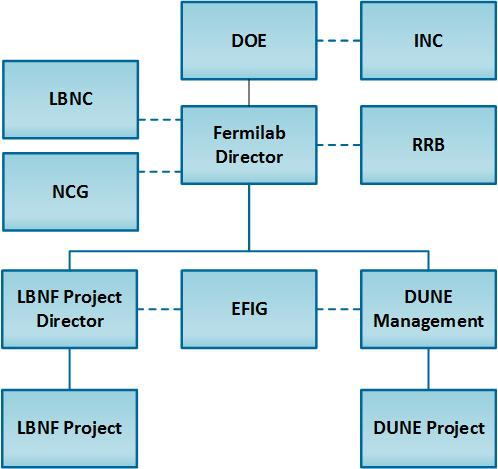
\includegraphics[width=0.65\textwidth]{lbnf_dune_org.jpg}
%\label{fig:mhexec}
\end{dunefigure}

\section{DUNE Organization and Management}

All aspects of DUNE are organized and managed by the DUNE collaboration.  Stakeholders include the collaborating institutions, the funding agencies participating in DUNE, and \fnal as the host laboratory.  All collaborating institutions have a representative on the DUNE Institutional Board (IB). The collaboration is responsible for the design, construction, installation, commissioning, and operation of the detectors and prototypes used to pursue the scientific program. The DUNE Executive Board (EB), described below, is the main management body of the collaboration and approves all significant strategic and technical decisions.

The top-level DUNE management team consists of two elected co-spokespersons, the technical coordinator (TC), and the resource coordinator (RC). The TC and RC are selected jointly by the co-spokespersons and the \fnal director. The management team is responsible for the day-to-day management of the collaboration, and for developing the overall collaboration strategy, which is presented for approval to the executive board. The executive board consists of the leaders of the main collaboration activities. The composition of the EB, currently including the DUNE management team, IB chair, physics coordinator, beam interface coordinator, computing coordinator, near detector coordinator, and leaders of the \dword{fd} consortia, described below, is intended to ensure
that all stakeholders in the collaboration have a voice in the decision-making process. 
In the post-TDR phase of DUNE, the intention is that the consortium leaders and the coordinators of the other major collaboration activities will become elected positions.
%, giving the full collaboration as a whole is represented in the decision-making process. 

To carry out design and construction work for the DUNE far detector, DUNE has  formed consortia of institutions that have taken responsibility for different detector subsystems. A similar structure will be formed for the DUNE near detector once the detector concept is selected. For the DUNE \dword{fd}, there are currently nine consortia, including three specific to \single, three specific to \dual, and three common to both technologies:
\begin{itemize}
\item (\single) \dwords{apa}, %Anode Plane Assemblies% (C. Touramanis, UK)
\item (\single) TPC \dword{ce}, % (D. Christian, US)
\item (\single) \dword{pds}, %Photon Detection System% (E. Segreto, Brazil)
\item (\dual) \dwords{crp}, %Charge Readout Planes% (D. Duchesneau, France)
\item (\dual) TPC electronics, %(D. Autiero, France)
\item (\dual) \dlong{pds} (PDS), %Photon Detection System %(I. Gil-Botella, Spain)
\item \dword{hv} system, %(F. Pietropaolo, CERN)
\item \dword{daq} system, %DAQ System %(D. Newbold, UK)
\item \dword{cisc} system. %Slow Controls and Instrumentation. %(S. Gollapinni, US)
\end{itemize}
It is possible that additional consortia may be added depending on the organization of computing and calibration systems. Each consortium has an overall leader, a technical lead, and a consortium board with representatives from each consortium institution. The consortia have full responsibility for their subsystems, including developing a full \dword{wbs}, understanding and documenting all interfaces with other systems, preparing final technical designs, and writing their respective sections of the \dword{tp} and the \dword{tdr}. Following approval of the  \dword{tdr}, they will be responsible for construction of their detector systems. %In addition to a variety of other tasks, the consortia are responsible for writing their respective sections of the technical proposal and the TDR.


%%%%%%%%%%%%%%%%%%%%%%%%%%%%%%%%%%%%%%%%%%%%%%%%%%%%%%%%%%%%%%% new 15 May
\section{Schedule and Milestones} 

%%%%% -- added
LBNF and DUNE are working toward three international project milestones:
\begin{itemize}
\item \maincavernstartexc{}: Start main cavern excavation in South Dakota; %at \surf{},
\item \firstfdmodstartinstall{}: Start installation of first \dword{fd} module; 
\item \beamturnon{}: Beam operation with two \dwords{detmodule}.
\end{itemize}
It is expected that these dates will be adjusted when the project baseline is defined. The key milestones to reach baseline status are:
\begin{itemize}
\item 2018 - Collect data with both \dword{protodune} detectors.
\item April 2019 - Submit \dword{tdr} for far \dwords{detmodule}.
\item July 2019 - Complete LBNC and NCG review of \dword{tdr}.
\item September 2019 - Present \dword{tdr} to RRB.
\item October 2019 - Conduct conceptual design (DOE CD-2/3b) review of LBNF and the USA scope of DUNE.
\end{itemize}
The \dword{tdr} for the near detector is expected to follow the \dword{fd} \dword{tdr} by approximately one year.

The schedule for the design and construction work for LBNF and DUNE has two critical parallel paths: one for the %Far Site scope at SURF 
far site (South Dakota) %(\surf) and %one 
another for the %Near Site scope at 
near site (Illinois). %(\fnal). 
The schedule for the initial work is driven by the \dword{cf} design and construction at each site.

During the initial phase of the project, the far site \dword{cf} is advanced first. The Ross Shaft rehabilitation
work at \surf was recently halted at the 4850L due to safety concerns, which have led to delays of two to four months. Early site preparation is timed to be completed 
in time to start excavation when the Ross Shaft rehabilitation work finishes. As each detector 
 cavern is excavated and sufficient utilities are installed, the cryostat and cryogenics system work proceeds, followed by detector installation, filling and commissioning. 
The first \dword{detmodule} is to be operational by 2024, with the second and third modules completed one and two years later, respectively.

The DOE project management process requires approvals at critical decision (CD) milestones that allow the LBNF/DUNE project to move to the next step. In spring 2018 LBNF near site \dword{cf} will seek CD-3b construction approval for Advanced Site Preparation to build the embankment. In 2020 LBNF and DUNE will seek to baseline the LBNF/DUNE scope of work, cost and schedule, as well as construction approval for the balance of the project scope of work. 

The project concludes with CD-4 approval to start operations.


%%%%%%%%%%%%%%%%%%%%%%%%%%%%%%%%%%%%%%%%%%%%%%%%%%%%%%%%%%%%%%
\section{The DUNE Technical Proposal Volumes}

%%%%%%%%%%%%%%%%%%%%%%%%%%%%%%%%%%%
%\subsection{A Roadmap of the TP}

The DUNE \dword{tp} describes the proposed physics program and 
technical designs of the far detector in preparation for the full \dword{tdr} 
to be published in 2019.  
It is intended as an intermediate
milestone on the path to a full \dword{tdr}, justifying the technical choices that flow down from the high-level physics goals through requirements at all levels of the Project. These design choices will enable the DUNE experiment to make the ground-breaking discoveries that will help to  answer %the flagship 
fundamental physics questions.

The  \dword{tp} is composed of three volumes. Volume 1 contains this executive summary, which describes 
the general aims of this document. The remainder of this first volume provides a more detailed description of the DUNE physics program that drives the choice of detector technologies. It also includes concise outlines of two overarching systems that have not yet evolved to consortium structures:  computing and calibration. 
%The second chapter summarizes DUNE's primary and ancillary science programs, and the third and fourth describe a computing and software model for DUNE and a possible calibration strategy, respectively, important topics that are under development in parallel with the detector development. % for the \lar \dwords{detmodule}.  
Volumes 2  and 3 describe, for the \single and \dual, %\dword{spmod} and the \dword{dpmod}, 
respectively, each module's subsystems, the technical coordination required for its design, construction, installation, and integration, and its organizational structure.



This \dword{tp}  represents the state of the design for the first three DUNE far detector modules at this moment
in time. The fourth module could employ a different \lartpc technology, taking into account  potential advances in technology to further optimize the sensitivity for physics discoveries. It is beyond the scope of this proposal. Also not covered in this proposal is the DUNE Near Detector, which constitutes an integral but less well developed portion of the experiment's  physics program. Separate \dwords{tdr}  for these detector systems will be
provided in the future.

